\chapter{Theory of Antenna Radiation}

\section{Radiation from a Conducting Rod}

A simple metallic rod can radiate electromagnetic energy when an alternating current (AC) is applied to it. The mechanism of radiation is fundamentally tied to the time-varying current along the conductor. Oscillating electrons within the rod generate a time-varying current, producing a time-varying electric field. According to Maxwell’s equations, this changing electric field creates a magnetic field, resulting in a propagating electromagnetic wave. A uniform, steady current will not radiate, whereas a current with spatial and temporal variation will. When the length of the rod is approximately half the wavelength of the incoming electric field, it becomes an efficient radiator, forming the well-known half-wave dipole.

\section{Transmission Lines and Directed Radiation}

Transmission lines, such as coaxial cables or parallel-wire lines, are engineered to transport electromagnetic energy with minimal loss while avoiding radiation. When the end of a transmission line is modified to open into free space, as in the case of a horn antenna, it can serve as a directional radiator. A horn antenna achieves this by gradually flaring the transmission line to match the impedance of free space.

\section{Dipole Antennas}

A dipole antenna consists of two conductive arms aligned end-to-end with a small feed gap. The alternating current through the arms produces radiated electromagnetic fields. The resulting pattern is typically doughnut-shaped, with maximum radiation perpendicular to the dipole axis and nulls along its length. For a half-wave dipole, each arm has length $\lambda/4$, giving a total dipole length of $\lambda/2$. The radiated power is described by the Poynting vector:
\[
\vec{S} = \vec{E} \times \vec{H}
\]
which represents the flow of electromagnetic energy away from the antenna.

\begin{figure}[H]
    \centering
    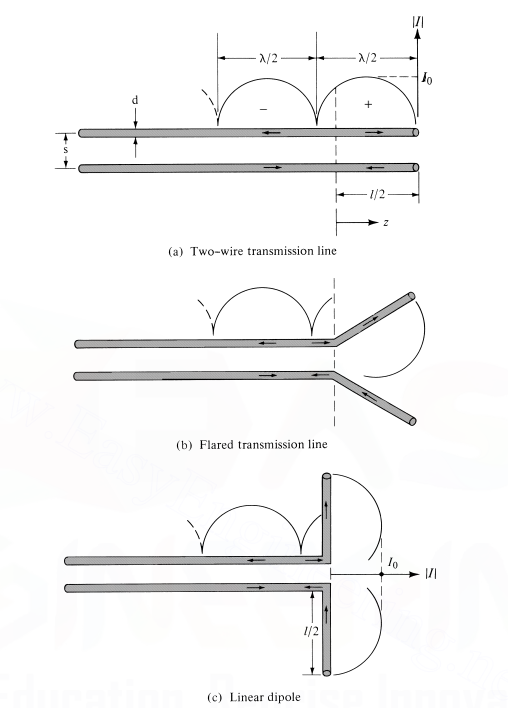
\includegraphics[width=0.75\textwidth]{figures/dipole.png}
    \caption{Current distribution on a lossless two-wire transmission line, flared transmission line, and linear dipole.}
    \small Image adapted from \cite{balanis}.
    \label{fig:dipole-current}
\end{figure}

\section{Isotropic Antennas and Radiation Parameters}

An isotropic antenna is a hypothetical point source that radiates equally in all directions, used as a reference for comparing real antennas. Its associated parameters include:

\begin{itemize}
    \item \textbf{Radiation intensity:}
    \[
    U(\theta,\phi) = r^2 S_r(\theta,\phi)
    \]
    where $S_r$ is the radial component of the Poynting vector.
    \item \textbf{Total radiated power:}
    \[
    P_{rad} = \int_{0}^{2\pi} \int_{0}^{\pi} U(\theta,\phi) \sin\theta \, d\theta \, d\phi
    \]
\end{itemize}

\section{Radiation Patterns and Beam Characteristics}

An antenna’s radiation pattern describes the spatial distribution of radiated power, typically represented in polar or 3D plots. These patterns help visualize how the antenna emits or receives energy in various directions.

Key features of a radiation pattern include:

\begin{itemize}
    \item \textbf{Main lobe}: The region of the radiation pattern that contains the direction of maximum radiation. This is typically aligned with the antenna’s boresight—defined as the axis or direction in which the antenna radiates most strongly.
    
    \item \textbf{Side lobes}: Smaller lobes that occur in directions away from the main beam. These represent unwanted radiation that can cause interference or reduce antenna efficiency.
    
    \item \textbf{Back lobe}: A specific side lobe that appears opposite to the main lobe, often minimized in directional antennas.
    
    \item \textbf{Nulls}: Directions in which the radiated power drops to zero or a local minimum. These are useful in applications like interference suppression or direction finding.
\end{itemize}

The \textbf{boresight} refers to the central axis of the main lobe—usually orthogonal to the plane of a symmetric antenna such as a dipole or horn. Beam steering, alignment, and antenna performance are often evaluated with respect to the boresight direction.

Radiation patterns can be analyzed by measuring or computing the far-field electromagnetic fields produced by the antenna. For electrically small antennas or arrays, Fourier transforms of the current distribution are commonly used to derive the angular power distribution.

\begin{figure}[H]
    \centering
    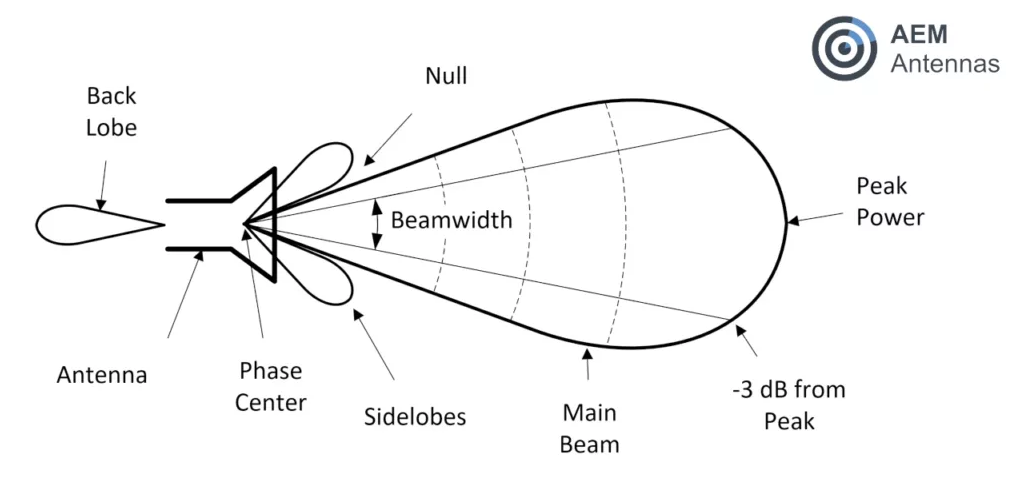
\includegraphics[width=0.7\textwidth]{figures/lobe.png}
    \caption{Visualization of an antenna radiation pattern showing the main lobe, side lobes, back lobe, and nulls.\\[0.5em]
    \small Image adapted from \cite{aemterms}.}
    \label{fig:lobes-pattern}
\end{figure}

\section{Beamwidth and Bandwidth}

Key parameters describing antennas include:
\begin{itemize}
    \item \textbf{HPBW (Half Power Beam Width)}:
    \[
    \theta_{HPBW} = \theta_2 - \theta_1, \quad \text{where } U(\theta_{1,2}) = 0.5 U_{max}
    \]
    \item \textbf{FNBW (First Null Beam Width)}: the angular separation between the first nulls on each side of the main lobe
\end{itemize}

\section{Gain and Directivity}

\begin{itemize}
    \item \textbf{Directivity}:
    \[
    D = \frac{4\pi U_{max}}{P_{rad}}
    \]
    \item \textbf{Gain}:
    \[
    G = \eta D
    \]
    where $\eta$ is the radiation efficiency, incorporating conductor or dielectric losses.
\end{itemize}
\section{S-Parameters in Antenna Design}

In high-frequency circuit analysis—including antenna systems—\textbf{S-parameters} (Scattering Parameters) are used to characterize how signals behave at the ports of a network. Figure~\ref{fig:sparams} illustrates a \textbf{2-port network}, which is a common model for analyzing antennas, filters, and other RF components.

\subsection*{S-Parameter Matrix Representation}

The network is described using incident and reflected wave amplitudes as follows:

\[
\begin{bmatrix}
b_1 \\
b_2
\end{bmatrix}
=
\begin{bmatrix}
S_{11} & S_{12} \\
S_{21} & S_{22}
\end{bmatrix}
\begin{bmatrix}
a_1 \\
a_2
\end{bmatrix}
\]

Where:
\begin{itemize}
    \item $a_1$, $a_2$ are the incident signals at Port 1 and Port 2, respectively,
    \item $b_1$, $b_2$ are the reflected signals from Port 1 and Port 2,
    \item $S_{ij}$ are the scattering parameters describing how input at Port $j$ affects output at Port $i$.
\end{itemize}

\subsection*{Definitions of Each S-Parameter}

From the figure:

\begin{align*}
S_{11} &= \frac{b_1}{a_1} \Big|_{a_2 = 0} \quad &\text{(Reflection at Port 1)} \\
S_{21} &= \frac{b_2}{a_1} \Big|_{a_2 = 0} \quad &\text{(Transmission from Port 1 to Port 2)} \\
S_{12} &= \frac{b_1}{a_2} \Big|_{a_1 = 0} \quad &\text{(Transmission from Port 2 to Port 1)} \\
S_{22} &= \frac{b_2}{a_2} \Big|_{a_1 = 0} \quad &\text{(Reflection at Port 2)}
\end{align*}

\subsection*{Interpretation in Antenna Context}

In antenna analysis (typically modeled as a 1-port network), the most relevant parameter is:

\[
S_{11} = \frac{V_{\text{reflected}}}{V_{\text{incident}}}
\]

\begin{itemize}
    \item $S_{11}$ quantifies how much power is reflected back from the antenna due to impedance mismatch.
    \item An $S_{11}$ value below $-10\,\mathrm{dB}$ implies that over 90\% of the input power is radiated or absorbed, which is generally considered acceptable.
\end{itemize}

\subsection*{Summary Table}

\begin{table}[H]
\centering
\caption{S-Parameter Definitions and Use in Antenna Design}
\begin{tabular}{lcl}
\toprule
\textbf{Parameter} & \textbf{Definition} & \textbf{Use} \\
\midrule
$S_{11}$ & $\frac{b_1}{a_1} \Big|_{a_2 = 0}$ & Return loss at Port 1 (antenna input) \\
$S_{21}$ & $\frac{b_2}{a_1} \Big|_{a_2 = 0}$ & Forward transmission (Port 1 to 2) \\
$S_{12}$ & $\frac{b_1}{a_2} \Big|_{a_1 = 0}$ & Reverse transmission (Port 2 to 1) \\
$S_{22}$ & $\frac{b_2}{a_2} \Big|_{a_1 = 0}$ & Return loss at Port 2 \\
\bottomrule
\end{tabular}
\end{table}

\begin{figure}[H]
\centering
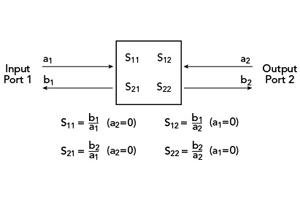
\includegraphics[width=0.55\textwidth]{figures/s11.jpg}
\caption{S-parameter model of a 2-port RF network showing definitions of $S_{ij}$ based on incident and reflected wave relationships.}
\small Image adapted from \cite{microwavejournal_sparams}.
\label{fig:sparams}
\end{figure}

\begin{figure}[H]
    \centering
    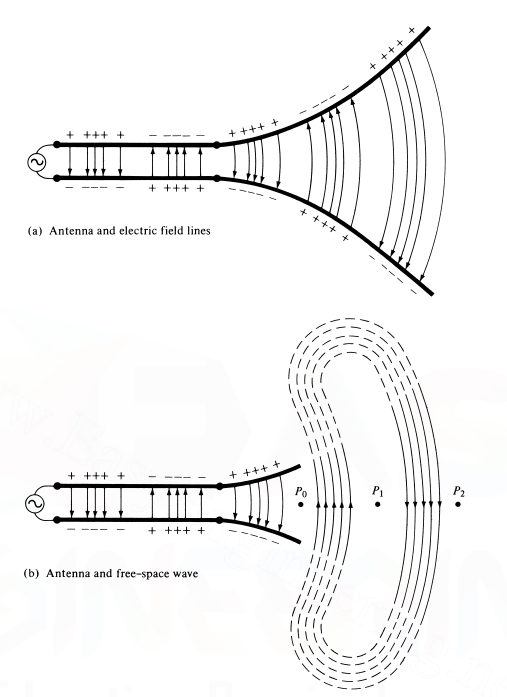
\includegraphics[width=0.6\textwidth]{figures/radiation.png}
    \caption{Source, transmission line, antenna, and detachment of electric field lines.}
    \small Image adapted from \cite{balanis}.
    \label{fig:radiation-overview}
\end{figure}

\section*{Conclusion}

This chapter provided a foundational understanding of antenna radiation by examining how time-varying currents generate electromagnetic fields and propagate energy through space. Key models such as dipole antennas and isotropic radiators were discussed, along with critical performance metrics including gain, directivity, beamwidth, and impedance characteristics.

While these theoretical principles help in designing efficient antennas under ideal conditions, real-world environments often introduce factors—such as weather, dust, or mechanical stress—that degrade antenna performance. This leads to the need for protective enclosures that can preserve radiation characteristics while shielding the antenna from external conditions.

In the next chapter, we introduce radomes: dielectric structures designed to protect antennas while maintaining electromagnetic transparency. We explore how their material properties, geometry, and placement can significantly impact the radiation behavior of enclosed antennas.

